% Created 2014-02-04 Tue 09:01
\documentclass[bigger]{beamer}
\usepackage[utf8]{inputenc}
\usepackage[T1]{fontenc}
\usepackage{fixltx2e}
\usepackage{graphicx}
\usepackage{longtable}
\usepackage{float}
\usepackage{wrapfig}
\usepackage{rotating}
\usepackage[normalem]{ulem}
\usepackage{amsmath}
\usepackage{textcomp}
\usepackage{marvosym}
\usepackage{wasysym}
\usepackage{amssymb}
\usepackage{hyperref}
\tolerance=1000
\usepackage{attrib}
\usepackage[autostyle]{csquotes}
\usepackage[backend=biber,style=authoryear-icomp,sortlocale=de_DE,natbib=true,url=false, doi=true,eprint=false]{biblatex}
\addbibresource{mybibfile.bib}
\usepackage{tikz}
\usetheme{Warsaw}
\author{Evan Misshula}
\date{2014-02-06 mon}
\title{Python interpreter and library management with pyenv}
\hypersetup{
  pdfkeywords={},
  pdfsubject={},
  pdfcreator={Emacs 24.3.2 (Org mode 8.2.5c)}}
\begin{document}

\maketitle
\begin{frame}{Outline}
\tableofcontents
\end{frame}


\section{Who is Evan Misshula?}
\label{sec-1}
\begin{frame}[label=sec-1-1]{Who is Evan Misshula?}
\begin{itemize}
\item @emisshula
\item EvanMisshula@gmail.com
\item \url{https://github.com/EvanMisshula}
\item \url{http://mofj.commons.gc.cuny.edu}
\item Evan Misshula on LinkedIn
\end{itemize}
\end{frame}
\section{What is a virtual environment and why do you want one?}
\label{sec-2}
\begin{frame}[label=sec-2-1]{What is a virtual environment and why do you want one?}
A virtual environment which allows you to work on a specific
project without worry of affecting other projects.(\href{http://docs.python-guide.org/en/latest/dev/virtualenvs/}{pydocs})
\begin{exampleblock}{New project requires Django 1.7, old one requires Django 1.5.}

\end{exampleblock}
\end{frame}
\begin{frame}[label=sec-2-2]{}
\begin{figure}[htb]
\centering
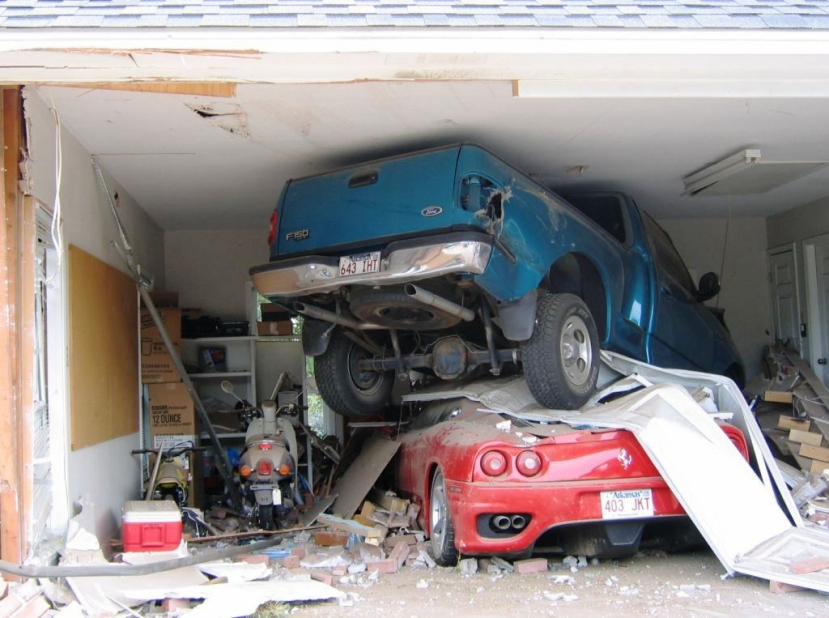
\includegraphics[width=.9\linewidth]{./images/2CarGarage1.jpg}
\caption{Unmanaged library conflict}
\end{figure}
\end{frame}

\begin{frame}[label=sec-2-3]{}
\begin{figure}[htb]
\centering
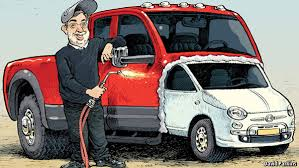
\includegraphics[width=.9\linewidth]{./images/TwoCars.jpeg}
\caption{Managed library conflict}
\end{figure}
\end{frame}

\section{What is a non-system version of python?}
\label{sec-3}
\begin{frame}[label=sec-3-1]{What is a \emph{non-system} version of python?}
For Linux and Mac OS X versions of python come pre-installed.  These 
lag the bleeding edge versions. 
\begin{exampleblock}{Upgrading by compiling from source can break your system.}
See stack overflow questions: 
\begin{itemize}
\item \href{http://stackoverflow.com/questions/18834381/i-broke-python-what-can-i-do}{I-broke-python},
\item \href{http://askubuntu.com/questions/333109/upgrading-to-python-2-7-5-on-ubuntu-12-04}{Upgrading-to-python-2.7.5}
\end{itemize}
\end{exampleblock}
\end{frame}
\begin{frame}[label=sec-3-2]{\emph{Non-system} version of python}
\begin{exampleblock}{Important libraries require a specific version of python}
critical features depend on the version for:
\begin{itemize}
\item Django (\href{https://docs.djangoproject.com/en/dev/faq/install/}{django-requires-2.7.x})
\item IPython (\href{http://ipython.org/faq.html}{IPython-requires-2.6.x})
\item pandas (\href{http://pandas.pydata.org/pandas-docs/stable/install.html#dependencies}{pandas-no-longer-supports-2.5.x})
\item matplotlib
\item scikit-learn
\item scipy.  (\href{http://stackoverflow.com/questions/3008509/python-version-2-6-required-which-was-not-found-in-the-registry}{required-python-version-not-found})
\end{itemize}
\end{exampleblock}
\end{frame}
\section{What is \href{https://github.com/yyuu/pyenv}{pyenv}?}
\label{sec-4}
\begin{frame}[label=sec-4-1]{What is \href{https://github.com/yyuu/pyenv}{pyenv}?}
Pyenv is a series of shell scripts that manage your python versions
through the use of \href{https://github.com/yyuu/pyenv#understanding-shims}{shims}. It does not depend on any version of
python and was forked from \href{https://github.com/sstephenson/rbenv}{rebenv}.
\end{frame}
\section{How do I use pyenv?}
\label{sec-5}
\begin{frame}[label=sec-5-1]{How do I use pyenv?}
\begin{itemize}
\item First install it (\href{http://mofj.commons.gc.cuny.edu/2014/01/20/ubuntu-set-up-a-virtual-environment-with-ipython-numpy-and-pandas/}{mine}, \href{http://askubuntu.com/questions/333109/upgrading-to-python-2-7-5-on-ubuntu-12-04}{KBowen} or \href{https://github.com/yyuu/pyenv#basic-github-checkout}{Yyuu})
\item Demo time\ldots{}
\end{itemize}
\end{frame}
\section{What is pyenv virtualenv?}
\label{sec-6}
\begin{frame}[label=sec-6-1]{What is pyenv virtualenv?}
\begin{itemize}
\item \href{https://github.com/yyuu/pyenv-virtualenv}{pyenv-virtualenv} is a \href{https://github.com/yyuu/pyenv}{pyenv} plugin that provides a 
pyenv virtualenv command to create virtualenv for 
Python on UNIX-like systems.
\end{itemize}
\end{frame}

\section{How do I use pyenv virtualenv?}
\label{sec-7}
\begin{frame}[label=sec-7-1]{How do I use pyenv virtualenv?}
\begin{itemize}
\item First install it (\href{http://mofj.commons.gc.cuny.edu/2014/01/20/ubuntu-set-up-a-virtual-environment-with-ipython-numpy-and-pandas/}{mine} or \href{https://github.com/yyuu/pyenv-virtualenv}{Yyuu-virtualenv})
\item Demo time
\end{itemize}
\end{frame}
\begin{frame}[label=sec-7-2]{}
\begin{figure}[htb]
\centering
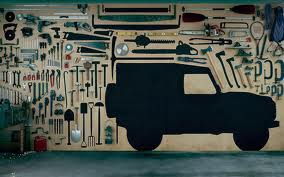
\includegraphics[width=.9\linewidth]{./images/garage.jpeg}
\caption{An organized work area}
\end{figure}
\end{frame}

\begin{frame}[label=sec-7-3]{}
\begin{figure}[htb]
\centering

\includegraphics[width=.9\linewidth]{./images/sepTools.jpeg}
\caption{An organized work area}
\end{figure}
\end{frame}
% Emacs 24.3.2 (Org mode 8.2.5c)
\end{document}